\documentclass[aspectratio=169]{beamer}
\usepackage[T1]{fontenc}
\usepackage[utf8]{inputenc}
\usepackage{lmodern}
\usepackage[french]{babel}
\usepackage{hyperref}
\usepackage{graphicx}
\usepackage{makecell}
\usepackage{xcolor}
\usepackage{colortbl}
\usepackage[flushleft]{threeparttable}

\graphicspath{ {./img/} }

%\newcommand{\TODO}{TODO:}
\newcommand*{\rot}{\rotatebox{90}}


% \title{Bacula\\~\\AIT --- Présentation}

\title{
    AIT --- Présentation \\~\\
    \centering
\includegraphics [height=20mm] {logo_bacula.png} 
}
% \titlegraphic{
\includegraphics [height=.2\textheight] {logo_bacula.png}}
\author{Gwendoline Dössegger, Noémie Plancherel, Gaby Roch, Cassandre Wojciechowski}
\author{Cassandre Wojciechowski \\ Gwendoline Dössegger \\ Noémie Plancherel \\ Gaby Roch}
\hypersetup{pdfauthor={G. Dössegger, N. Plancherel, G. Roch, C. Wojciechowski}}
\date{8 novembre 2021}

\begin{document}

\begin{frame}
  \titlepage
\end{frame}

\begin{frame}{Bacula -- Présentation générale}
 \begin{itemize}
  \item Logiciel de sauvegarde multi-platform créé en 2000 par Kern Sibbald
  \item Première version 2002
  \item Dernière version 11.0.5, juin 2021
  \item Open source / private source
 \end{itemize}
\end{frame}

\begin{frame}{Architecture}
  \begin{center}
    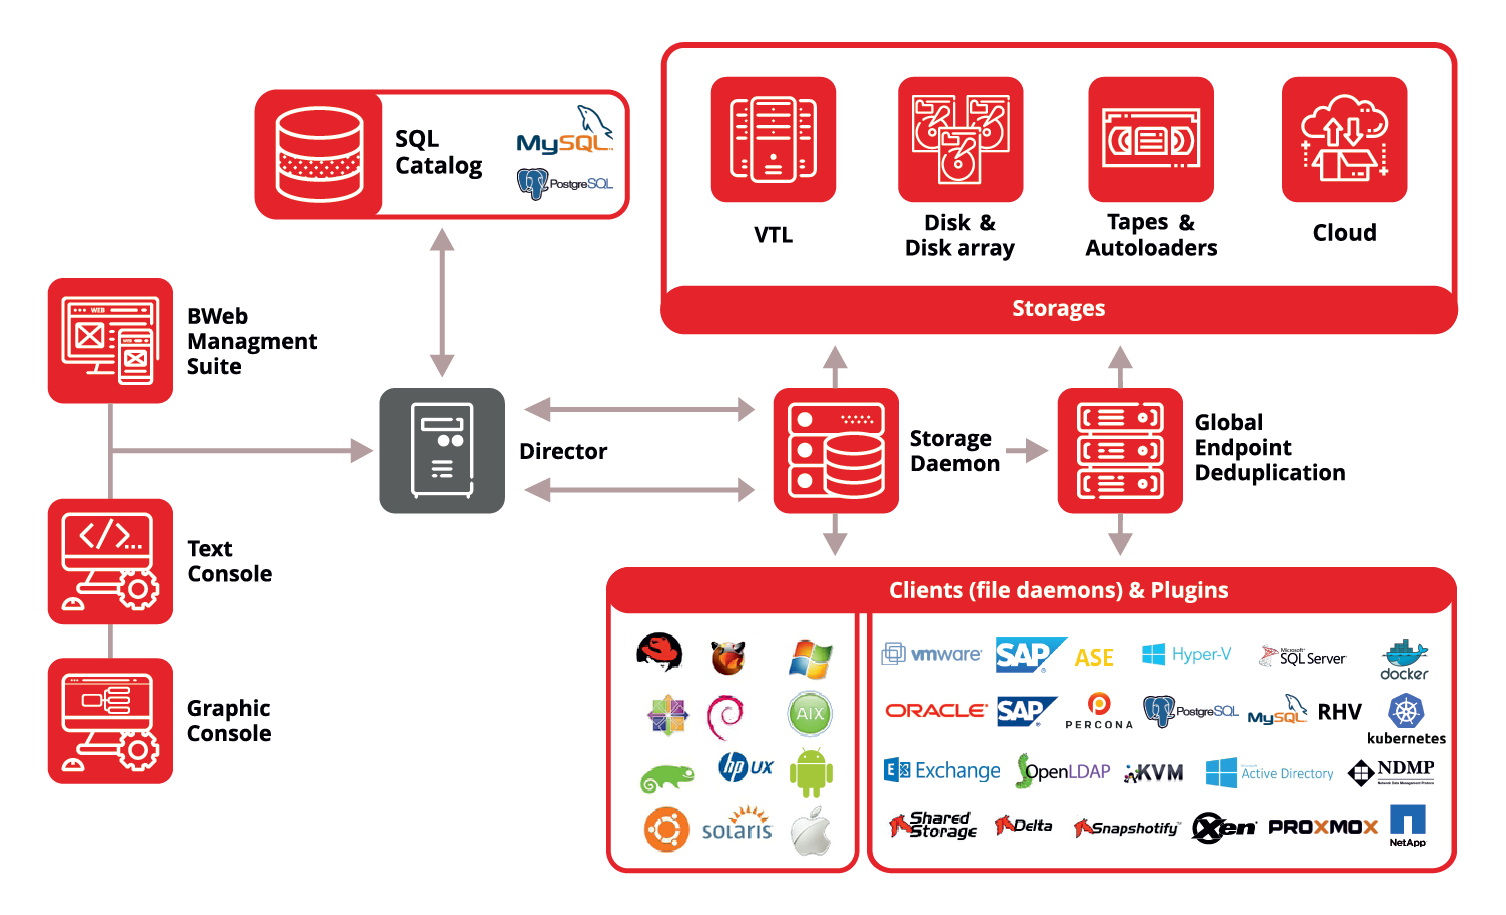
\includegraphics[height=80mm]{architecture.png}
  \end{center}  
\end{frame}

\begin{frame}{Architecture}
 \begin{itemize}
  \item Chiffrement et signature des backups possible
  \item La master key doit être sauvegardée manuellement hors-site
  \item S'il y a perte de la master key, les backups sont perdus
 \end{itemize}
\end{frame}

\begin{frame}{Démonstration}
\end{frame}

\begin{frame}{CPU}
\begin{center}
  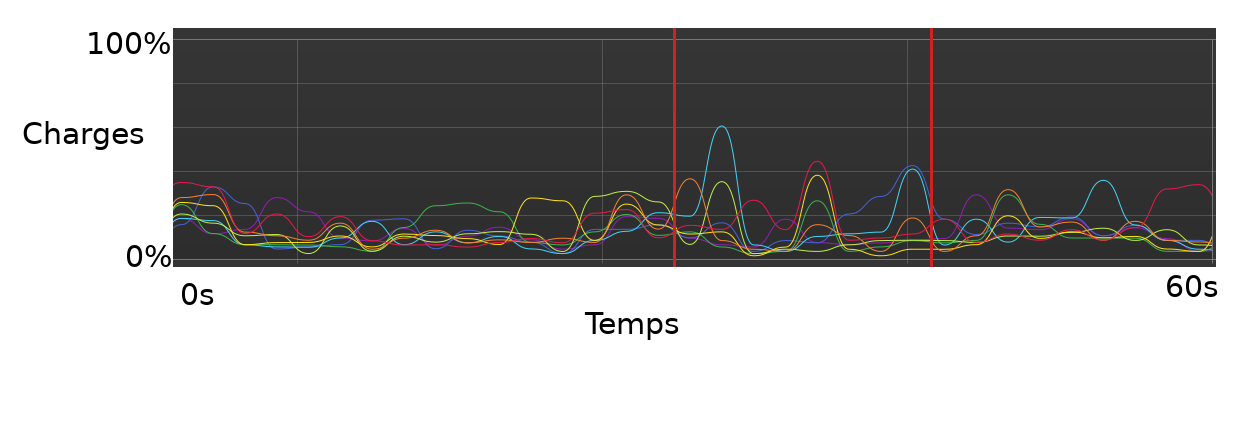
\includegraphics[height=30mm]{graphCPU}
\end{center}
\end{frame}

\begin{frame}{Coûts}
\begin{center}

\begin{itemize}
    \item 2 versions: Community Open Source et Entreprise
    \item La version Entreprise propose (entre autres) un expert qui permet d'apporter un support technique
    \item Dès 500\$ par mois sur devis pour la version Entreprise (abonnement Standard)
\end{itemize}

 \begin{tabular}{|l|ccccc|}
    \hline
    & Standard & Bronze & Silver & Gold & Platinum \\
    \hline
    \hline
    Nombre de clients & < 50 & < 200 & < 500 & < 2000 & < 5000 \\
    \hline
    Nombre de contacts & 1 & 2 & 3 & 5 & 5 \\
    \hline
    Assistance & Web & Web & Web et tél.& Web et tél. & Web et tél. \\
    \hline
    Nombre d'OS & 4 & toutes & toutes & toutes & toutes \\
    \hline
    Temps de réponse & 1j -- 4j & 6h -- 4j & 4h -- 2j & 1h -- 2j & 1h -- 2j \\ %heure/jour ouvrable
    du support &  & & & & \\
    \hline
    Formation & 0 & 0 & 0 & 0 & 1/an \\
    \hline
 \end{tabular}
\end{center}
\end{frame}


\begin{frame}{Comparaison}
 \begin{center}
  \begin{tabular}{|l||c|c|c|c|c|c|c|c|c|c|}
    \hline
    & Coût & \rot{Open source ~} & Backups & \rot{Déduplication ~} & \rot{Chiffrement ~} & \rot{Compression ~} & \rot{Web interface} & \rot{Linux} & \rot{MacOS X} & \rot{Windows} \\
    \hline
    \hline
    Bacula & \makecell{Gratuit\\Payant} & \cellcolor{green!50} & \makecell{Full\\ Incrémentaux\\ Différentiels} & \cellcolor{green!50} & \cellcolor{green!50} & \cellcolor{green!50} & \cellcolor{green!50} & \cellcolor{green!50} & \cellcolor{green!50} & \cellcolor{green!50} \\
    \hline
    BorgBackup & \makecell{Gratuit\\Payant} & \cellcolor{green!50} & \makecell{Full\\ Incrémentaux\\ Différentiels} & \cellcolor{green!50} & \cellcolor{green!50} & \cellcolor{green!50} & \cellcolor{orange!50} & \cellcolor{green!50} & \cellcolor{green!50} & \cellcolor{red!50} \\
    \hline
    Bup & Gratuit & \cellcolor{green!50} & Incrémentaux & \cellcolor{green!50} & \cellcolor{red!50} & \cellcolor{green!50} & \cellcolor{green!50} & \cellcolor{green!50} & \cellcolor{green!50} & 
    \cellcolor{red!50} \\
    \hline
    Duplicati & Gratuit & \cellcolor{green!50} & \makecell{Full\\ Incrémentaux} & \cellcolor{green!50} & \cellcolor{green!50} & \cellcolor{green!50} & \cellcolor{green!50} & \cellcolor{green!50} & \cellcolor{green!50} & \cellcolor{green!50} \\
    \hline
    Rsync & Gratuit & \cellcolor{green!50} & Incrémentaux & \cellcolor{red!50} & \cellcolor{red!50} & \cellcolor{red!50} & \cellcolor{red!50} & \cellcolor{green!50} & \cellcolor{green!50} & \cellcolor{green!50}  \\
    \hline
 \end{tabular}
 \begin{tablenotes}
 \scriptsize 
  \fcolorbox{black}{green!50}{\rule{0pt}{4pt}\rule{4pt}{0pt}}\quad Oui \fcolorbox{black}{red!50}{\rule{0pt}{4pt}\rule{4pt}{0pt}}\quad Non
  \fcolorbox{black}{orange!50}{\rule{0pt}{4pt}\rule{4pt}{0pt}}\quad En développement
    \end{tablenotes}
 \end{center}
\end{frame}

\begin{frame}{Avantages / inconvénients}
    \begin{center}
     \begin{tabular}{|l|l|}
     \hline
      \textbf{Avantages} & \textbf{Inconvénients} \\
     \hline
     \hline
        Interface utilisateur graphique & Prise en main complexe (fichiers \\ 
                                        & de configuration) \\
     \hline
     Cross-platform & Pas de scan de virus \\
     \hline
     Automatisation \& planification des tâches & Configuration nécessaire au backup \\ 
                                                & des appareils mobiles\\
     \hline
     Sauvegarde continue (CDP) & \\
     \hline
     Toujours maintenu (dernière update : juin 2021) & \\
     \hline
     Sauvegarde Cloud \& hors-site & \\
     \hline
     Charge réseau \& CPU modulables & \\
     \hline
     Déduplication des données & \\
     \hline
     Support d'environnements virtuels & \\
     \hline
     Large documentation et en plusieurs langues & \\
     \hline
     \end{tabular}

    \end{center}

\end{frame}

\begin{frame}{Conclusion}
 \begin{itemize}
  \item Sauvegarde jusqu'à 1x par heure - RPO très faible
  \item Automatisation et planification possibles
  \item Economie de temps, d'argent, de stress
 \end{itemize}
\end{frame}

\begin{frame}{Questions ?}
  \begin{center}
    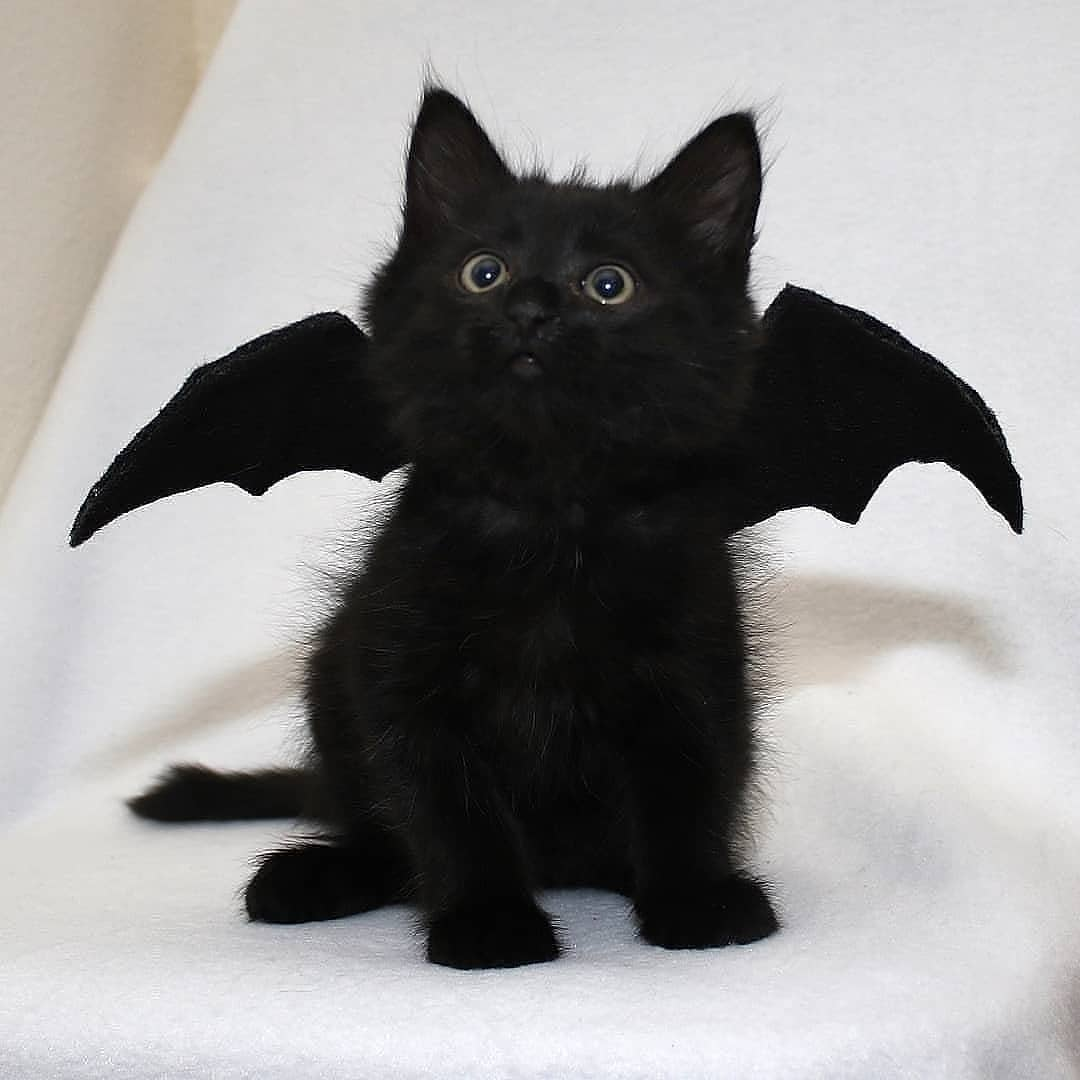
\includegraphics[height=60mm]{bat_kitty.jpg}
  \end{center}  
\end{frame}


\end{document}
